% Architecture diagram for "Ordinal Capsule Regression on Retinal Foundation Features".
% Standalone TikZ. Compiles to a single-page, tightly-cropped PDF that drops in as
% 
\includegraphics[width=\columnwidth]{figs/fig_architecture.pdf}.

\documentclass[tikz, border=3mm]{standalone}

\usepackage{amsmath,amssymb}
\usepackage[T1]{fontenc}
\usepackage{helvet}
\renewcommand{\familydefault}{\sfdefault}

\usetikzlibrary{positioning, arrows.meta, fit, calc, backgrounds, shapes.geometric}

\definecolor{colFrozen}{HTML}{E0E3E7}
\definecolor{colFrozenEdge}{HTML}{7A8290}
\definecolor{colTrainable}{HTML}{FFF2C4}
\definecolor{colTrainableEdge}{HTML}{D9A441}
\definecolor{colHead}{HTML}{FFDCC4}
\definecolor{colHeadEdge}{HTML}{E38050}
\definecolor{colInput}{HTML}{DCE7F5}
\definecolor{colInputEdge}{HTML}{7090C0}
\definecolor{colPrep}{HTML}{E7DCF2}
\definecolor{colPrepEdge}{HTML}{8A75B5}
\definecolor{colOutput}{HTML}{D7EED8}
\definecolor{colOutputEdge}{HTML}{5BA560}
\definecolor{colUQ}{HTML}{F6D8D8}
\definecolor{colUQEdge}{HTML}{C26A6A}
\definecolor{colLoRA}{HTML}{C62E4B}

\begin{document}
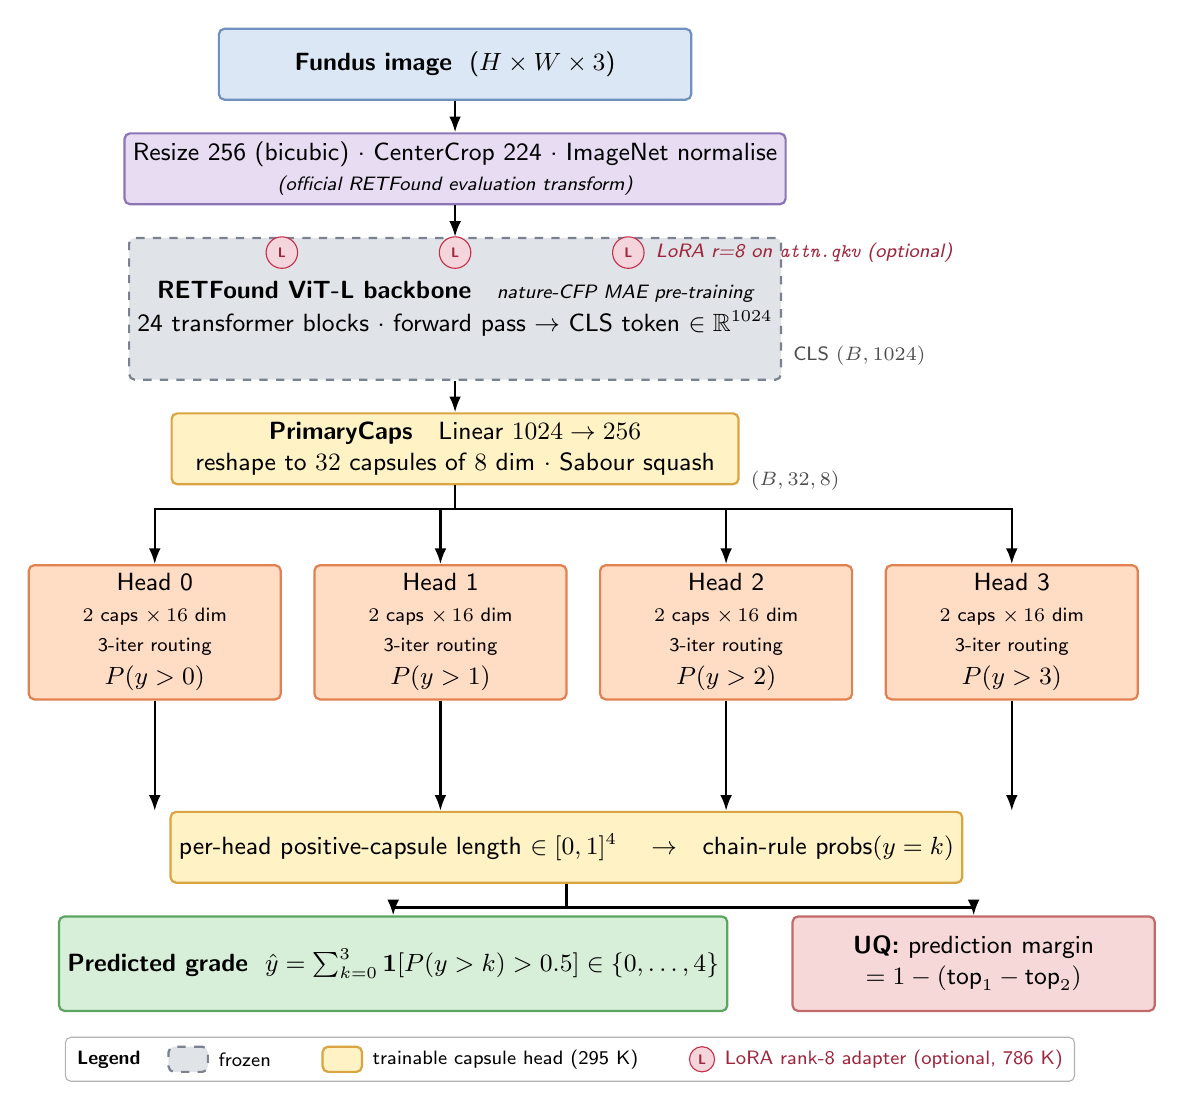
\begin{tikzpicture}[
    font=\small,
    >={Latex[length=2mm]},
    node distance=4mm and 4mm,
    box/.style={draw, thick, rounded corners=2pt, align=center,
                inner sep=3pt, minimum height=9mm},
    input/.style={box, fill=colInput,   draw=colInputEdge},
    prep/.style={box, fill=colPrep,    draw=colPrepEdge,    minimum width=72mm},
    frozen/.style={box, fill=colFrozen, draw=colFrozenEdge, dashed, minimum width=80mm, minimum height=18mm},
    trainable/.style={box, fill=colTrainable, draw=colTrainableEdge, minimum width=72mm},
    head/.style={box, fill=colHead, draw=colHeadEdge, minimum width=32mm, minimum height=14mm},
    output/.style={box, fill=colOutput, draw=colOutputEdge, thick, minimum width=72mm, minimum height=12mm},
    uqbox/.style={box, fill=colUQ, draw=colUQEdge, minimum width=46mm, minimum height=12mm},
    arr/.style={->, thick},
    lbl/.style={font=\scriptsize\itshape, text=black!55, inner sep=1pt},
    tag/.style={font=\scriptsize, text=black!70, inner sep=1pt},
    lora/.style={circle, draw=colLoRA, fill=colLoRA!20,
                 minimum size=4mm, inner sep=0pt, font=\tiny\bfseries, text=colLoRA!80!black},
]

% ---- Main vertical flow ----------------------------------------------------
\node[input, minimum width=60mm] (img) {\textbf{Fundus image} \ ($H\times W\times 3$)};

\node[prep, below=of img] (pp) {%
    Resize 256 (bicubic) $\cdot$ CenterCrop 224 $\cdot$ ImageNet normalise\\%
    {\scriptsize\itshape (official RETFound evaluation transform)}};

\node[frozen, below=of pp] (vit) {%
    \textbf{RETFound ViT-L backbone}\quad{\scriptsize\itshape nature-CFP MAE pre-training}\\[1pt]%
    24 transformer blocks  $\cdot$  forward pass  $\to$  CLS token $\in \mathbb{R}^{1024}$};

% LoRA adapter markers tucked into the ViT box
\node[lora, xshift=-22mm, yshift=-2mm] at (vit.north) (lora1) {L};
\node[lora, xshift=0mm,   yshift=-2mm] at (vit.north) (lora2) {L};
\node[lora, xshift=22mm,  yshift=-2mm] at (vit.north) (lora3) {L};
\node[lbl, right=1mm of lora3, text=colLoRA!80!black]
    {\scriptsize LoRA r=8 on \texttt{attn.qkv} (optional)};

\node[trainable, below=of vit] (pc) {%
    \textbf{PrimaryCaps}\quad Linear $1024 \to 256$\\%
    reshape to $32$ capsules of $8$ dim  $\cdot$  Sabour squash};

% ---- Four ordinal DigitCaps heads ------------------------------------------
\node[head, below left =10mm and 22mm of pc.south] (h0) {Head 0\\\scriptsize $2$ caps $\times\,16$ dim\\\scriptsize 3-iter routing\\[1pt] $P(y>0)$};
\node[head, right=4mm of h0]               (h1) {Head 1\\\scriptsize $2$ caps $\times\,16$ dim\\\scriptsize 3-iter routing\\[1pt] $P(y>1)$};
\node[head, right=4mm of h1]               (h2) {Head 2\\\scriptsize $2$ caps $\times\,16$ dim\\\scriptsize 3-iter routing\\[1pt] $P(y>2)$};
\node[head, right=4mm of h2]               (h3) {Head 3\\\scriptsize $2$ caps $\times\,16$ dim\\\scriptsize 3-iter routing\\[1pt] $P(y>3)$};

% ---- Combiner + outputs ----------------------------------------------------
\node[trainable, below=14mm of h1.south, minimum width=80mm,
      xshift=16mm] (comb)
    {per-head positive-capsule length $\in [0,1]^{4}$ \quad$\to$\quad chain-rule probs$(y=k)$};

\node[output, below=of comb, xshift=-22mm, minimum width=58mm] (pred)
    {\textbf{Predicted grade} $\ \hat{y} = \sum_{k=0}^{3} \mathbf{1}[P(y>k) > 0.5] \in \{0,\dots,4\}$};

\node[uqbox, right=8mm of pred] (uq)
    {\textbf{UQ:} prediction margin\\$= 1 - (\text{top}_1 - \text{top}_2)$};

% ---- Arrows ----------------------------------------------------------------
\draw[arr] (img)  -- (pp);
\draw[arr] (pp)   -- (vit);
\draw[arr] (vit)  -- (pc);
\draw[arr] (pc.south) -- ++(0,-3mm) -| (h0.north);
\draw[arr] (pc.south) -- ++(0,-3mm) -| (h1.north);
\draw[arr] (pc.south) -- ++(0,-3mm) -| (h2.north);
\draw[arr] (pc.south) -- ++(0,-3mm) -| (h3.north);
\draw[arr] (h0.south) -- (h0.south |- comb.north);
\draw[arr] (h1.south) -- (h1.south |- comb.north);
\draw[arr] (h2.south) -- (h2.south |- comb.north);
\draw[arr] (h3.south) -- (h3.south |- comb.north);
\draw[arr] (comb.south) -- ++(0,-3mm) -| (pred.north);
\draw[arr] (comb.south) -- ++(0,-3mm) -| (uq.north);

% ---- Shape/tensor annotations on arrows ------------------------------------
\node[tag, right=1mm of vit, yshift=-6mm] {\scriptsize CLS $(B, 1024)$};
\node[tag, right=1mm of pc,  yshift=-4mm] {\scriptsize $(B, 32, 8)$};

% ---- Legend (placed below the whole diagram; bounding box auto-sized) ------
% We place each legend item first, then draw the bounding rectangle on the
% background layer with fit= over all items. This guarantees the grey border
% wraps every swatch + label exactly, rather than being clipped on the right.
\coordinate (legAnchor) at ([yshift=-6mm]pred.south west);

\node[anchor=west, font=\scriptsize, inner sep=1pt] (leg-label)
      at ([xshift=2mm]legAnchor) {\textbf{Legend}};

\node[box, fill=colFrozen, draw=colFrozenEdge, dashed,
      minimum width=5mm, minimum height=3.2mm, inner sep=0pt,
      right=3mm of leg-label.east, anchor=west] (sw1) {};
\node[anchor=west, font=\scriptsize, inner sep=1pt] (sw1lbl)
      at ([xshift=0.8mm]sw1.east) {frozen};

\node[box, fill=colTrainable, draw=colTrainableEdge,
      minimum width=5mm, minimum height=3.2mm, inner sep=0pt,
      right=6mm of sw1lbl.east, anchor=west] (sw2) {};
\node[anchor=west, font=\scriptsize, inner sep=1pt] (sw2lbl)
      at ([xshift=0.8mm]sw2.east) {trainable capsule head (295 K)};

\node[lora, minimum size=3.2mm, right=6mm of sw2lbl.east, anchor=west] (sw3) {L};
\node[anchor=west, font=\scriptsize, inner sep=1pt, text=colLoRA!80!black] (sw3lbl)
      at ([xshift=0.8mm]sw3.east) {LoRA rank-8 adapter (optional, 786 K)};

\begin{scope}[on background layer]
\node[draw=black!30, rounded corners=2pt, inner sep=3pt,
      fit=(leg-label) (sw1) (sw1lbl) (sw2) (sw2lbl) (sw3) (sw3lbl)] {};
\end{scope}

\end{tikzpicture}
\end{document}
